\documentclass[UTF8]{scrartcl}

\usepackage{xeCJK}
\usepackage{graphicx}
\usepackage{subfigure}
\usepackage{indentfirst}
\setlength{\parindent}{2em}
\usepackage{listings}


\lstset{
	columns=fixed,       
	frame=none,                                          % 不显示背景边框
	%backgroundcolor=\color[RGB]{0,0,0},            % 设定背景颜色
	keywordstyle=\color[RGB]{40,40,255},                 % 设定关键字颜色
	numberstyle=\footnotesize\color{darkgray},           
	commentstyle=\it\color[RGB]{0,96,96},                % 设置代码注释的格式
	stringstyle=\rmfamily\slshape\color[RGB]{128,0,0},   % 设置字符串格式
	showstringspaces=false,                              % 不显示字符串中的空格
	language=c++,                                        % 设置语言
}



%opening
\title{Dataflow问题}
\author{}

\begin{document}

\maketitle


\section{问题描述}

以一个简单的1D卷积为例,卷积核为2x1,输入为3x1,输出为2x1,其计算伪代码如下所示:

\begin{lstlisting}

                    Loopi: for(i=0; i<2; i++){
                          Loopj:for(j=0; j<2; j++){
	                            O[i] += K[j] * I[j+i];
                                 }
                           }
                                     
\end{lstlisting}

\section{Graph变换}

	将上述计算完全展开可显示其可并行性和数据依赖。如Figure 1 所示,K1、K2和I2 存在数据复用的机会,计算完全并行时需要4个乘法器和2个加法器。实际情况中,由于计算资源和访存带宽的限制并不能将计算完全并行化,同时考虑到能耗的限制,需要充分利用计算中数据复用的机会,减少从外部存储读取数据。假设PE单元数目为2,下面给出NO Local Reuse和Weight Stationary时的分析。
	
			\begin{figure}[h]
				\centering
				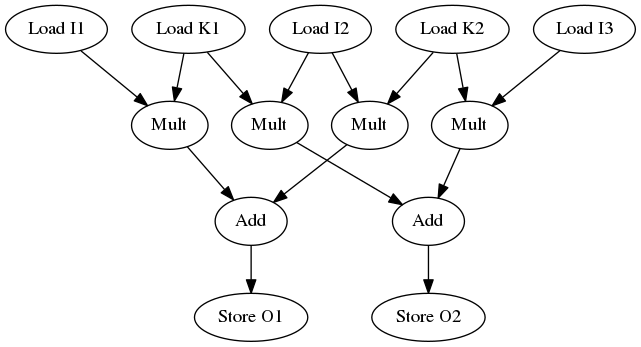
\includegraphics[width=3.0in,height=1.8in]{ws.png} 
				\caption{Origin Graph}
				\label{fig1}
			\end{figure}

	\subsection{No Local Reuse}
	
		Figure 2(a) 是No Local Reuse的graph表示图,从图中可以看出,由于硬件资源限制,内层循环被展开并行执行,外层循环顺序执行。由于没有local register(Local Reuse),外层循环的计算每次都需要重新读入权重和输入数据。
		
	
	\begin{figure}[h]
		\centering
		\subfigure[No Local Reuse]{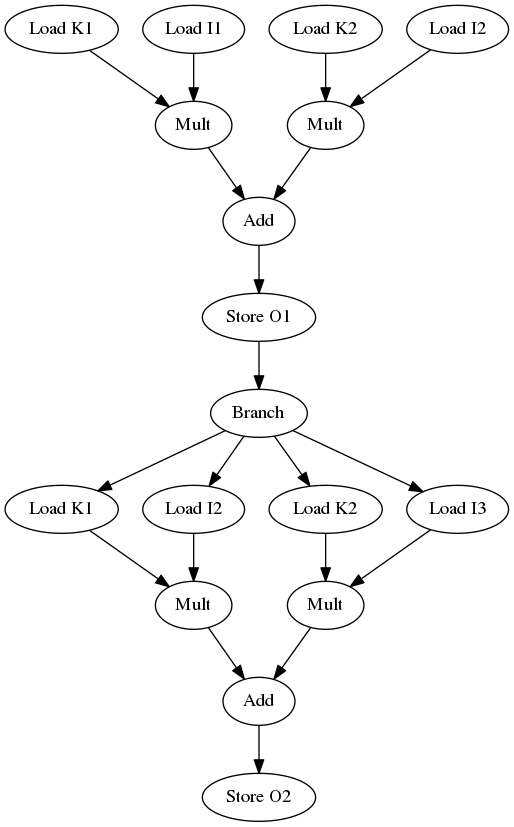
\includegraphics[width=1.40in,height=3.0in]{nlr.png} }
		\subfigure[Weight Stationary]{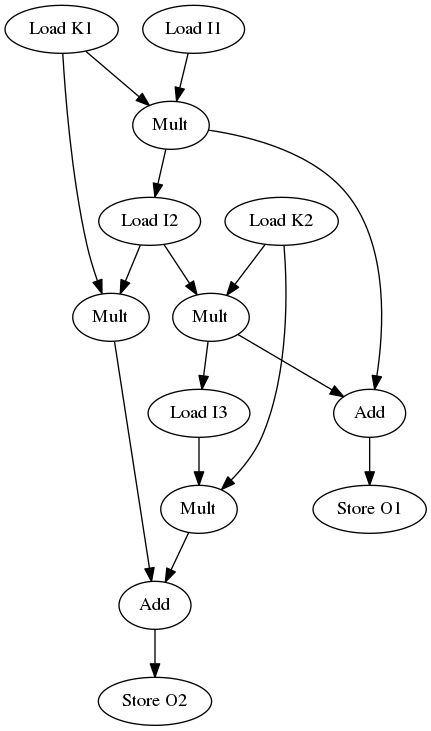
\includegraphics[width=1.40in,height=3.0in]{ws_s.png} }
		\caption{Transformed Graph}
		\label{fig2}
	\end{figure}
	
	
	\subsection{Weight Stationary}
	   Figure 2(b)是 Weight Stationary 的graph表示图。从图中可以看出,权重被load一次后即存在PE中被复用,I1、I2、I3依次读入并广播至所有PE分别与权重数据进行计算。按照Aladdin的策略Schedule该graph,依次执行的计算是(I1×K1)(I2xK1, I2xK2, o1=I1xk1+I2xK2)(I3xK2, 02=I2xK1+I3xK2)。即Oi的部分和I1xK1在第一个cycle的PE1中计算,I2xK2在下一个cycle的PE2中计算,同时在第二个cycle将PE1中的输出传入PE2做累加,如此流水进行。
	   
	   相比较NLR,WS的latency增大,即每个output需要两个cycle计算,但由于存在local的数据复用,减少了从buffer读取数据的次数。
	   


\end{document}